Här följer de resultat som vi har som vi samlat in under studien. De innehåller dels resultaten från den enkät som delas ut vid två tillfällen till gruppen. Vi tar även upp våra egna observationer över hur inlärningen har utvecklats med tiden. 


\subsection{Git i agila utvecklingsprojekt}
Av de observationer som vi har kunnat göra iform utav coacher har vi kommit framtill att vi ser tydliga framsteg både i förståelsen för hur ett projekt av större storlek fungerar och vilka nya problem som uppstår. Framför allt så har vi observerat att studenterna ser stor nytta av ett versionshatneringssystem och den gemensamma uppfattningen är att Git fungerar väldigt bra. Vi själva tycker att problemen kring verktyget är få och förhållande små. Då vi pratar med andra grupper, som läser samma kurs, så framgår det tydligt att vi har mycket mindre problem. Detta tror vi dels för att Git har mycket bättre merge-vertyg och att vi inte använder oss utav något eclipse plugin. Eftersom vi använder git i terminalen får vi även en effekt av att man tänker till en extra gång innan man gör något. Vi tror att det är bra och tror inte att det leder till att man sprider sin kod mer sällan utan att utvecklarna tänker till innan och inte sprider felaktig kod lika ofta. 

Vi ser att git växer mer och mer i de framtidsrapport vi har studerat och en intressant tanke för kursen skulle vara att ersätta CVS/SVN med Git. Gruppen utvecklar i Eclipse som IDE, och den senaste versionen av programmet kommer med en mycket uppskattad version av EGit/JGit. Vi coacher har testat detta och ser fördelarna med att använda ett grafiskt plugin för att underlätta för utvecklarna. Den förberedande laborationen, se figur \ref{fig:Timeline} , skulle då inrikta sig på att lära ut Egit. Problemet på denna lösning är att Instutitionen förnärvarande endast levererar en Eclipse version som är två versioner bakom. 


\subsection{Utveckling}
\subsection{Enkätundersökning}

\begin{figure}[htb!]\centering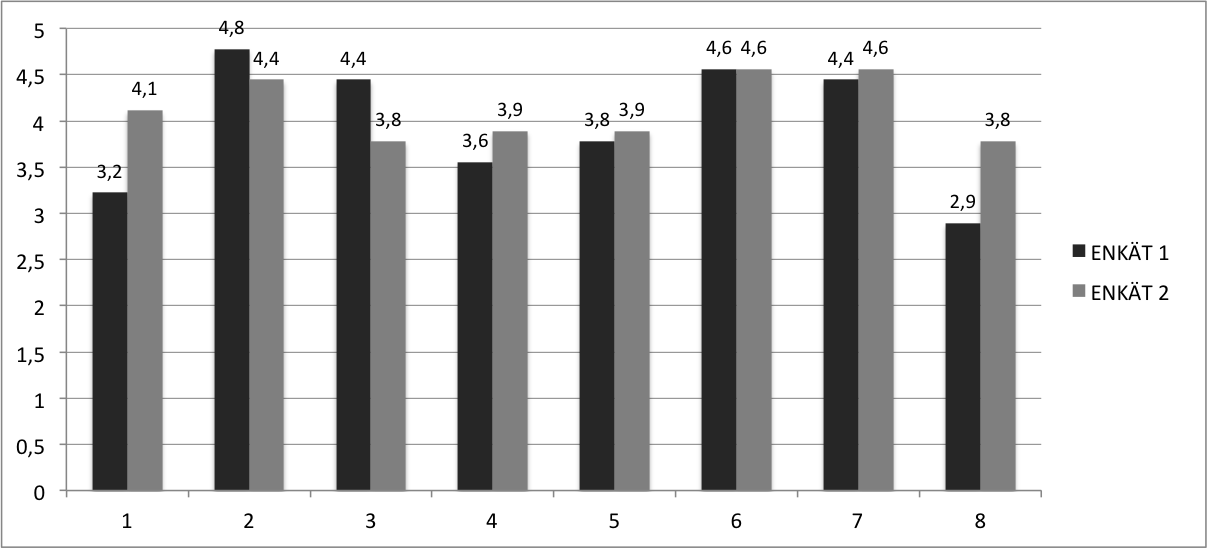
\includegraphics[width=0.75\textwidth]{EnkatResultatMindre.png}\caption{Visar upplägget i ett centraliserat versionshanteringssytem. Alla användare kopplar upp sig mot ett gemensamt repo}\label{fig:enkat}\end{figure}

Här följer de frågor som fanns med i enkäten som delades ut samt en kort diskussion om resultaten.

\subsubsection{Snabbguiden gjorde det enkelt att förstå grunderna i Git}

\subsubsection{Det är lätt att få igång ett bra workflow (liknande update, update, update, commit för SVN)}


\subsubsection{Att använda Terminalen gör att man förstår bättre hur Git fungerar}


\subsubsection{Git hanterar mergkonflikter på ett bra sätt}


\subsubsection{Git fungerar bra tillsammans med Eclipse}


\subsubsection{När vi stöter på problem med Git kan ni som coacher ofta lösa det}


\subsubsection{Mitt helhetsintryck av Git är att det är ett bra versionshanteringssystem}


\subsubsection{Jag kommer fortsätta använda Git som versionshanteringssystem}
